% GECCO 2027 full paper. Template line follows the GECCO paper submission instructions.
% Limits: 8 pages excluding references; abstract at most 200 words; double blind.
% Source comments of the form "% src:" name the record each number came from.
% GECCO's submission header adds review=true, which prints line numbers for reviewers.
% It is off while drafting; add it back to the options below when submitting.
% GECCO review is double blind: also add anonymous=true when submitting, which hides
% the author block below.
\documentclass[dvipsnames,format=sigconf]{acmart}

\usepackage{algorithm}
\usepackage{algpseudocode}
\usepackage{dsfont}
\usepackage{tikz}
\usetikzlibrary{positioning,arrows.meta,fit,calc}

\setcopyright{none}
\settopmatter{printacmref=false}
\renewcommand\footnotetextcopyrightpermission[1]{}
\acmConference[GECCO '27]{Genetic and Evolutionary Computation Conference}{July 12--16, 2027}{Krakow, Poland}
\acmYear{2027}

\newcommand{\ind}{\mathds{1}}
\newcommand{\cmaes}{CMA-ES}

\begin{document}

\title{Evolve, Don't Retrain: Safety Adapters for Frozen World Models}

\author{Sachin Mohan}
\email{sachinmohan29@gmail.com}
\affiliation{%
  \institution{University of the Witwatersrand}
  \city{Johannesburg}
  \country{South Africa}}

\begin{abstract}
Planners built on learned world models can finish long tasks from pixels, but nothing in
their cost tells them what to avoid. The usual fixes need tuned penalties or hand-written
rules. Evolution needs only a ranking, so safety can simply come first. We state the
problem as a constrained Markov decision process and propose a framework that evolves a
thin adapter around a frozen planner. The adapter starts as an exact identity, candidates
are ranked by safe completions, then completions, then fewer violations, and the best is
locked before any held-out case is seen. On TwoRoom navigation, CMA-ES adapters scored above
the bare planner in all nine held-out searches, at about twice its safe completion, and
above random search in seven of nine repeats. PPO at its frozen settings barely moved. The
gains have limits: exploratory intervals include zero, unselected adapters reached 13 to
16\%, violations did not fall reliably, and random search scored as high in one run. On
simulated Block Plucking, an evolved selector showed no signal over 48 starts. Evolution can
use this adapter slot on TwoRoom, but differences between repeats and layouts can be as large
as those between search methods.
\end{abstract}

\begin{CCSXML}
<ccs2012>
<concept>
<concept_id>10010147.10010257.10010293.10011809</concept_id>
<concept_desc>Computing methodologies~Bio-inspired approaches</concept_desc>
<concept_significance>500</concept_significance>
</concept>
<concept>
<concept_id>10010147.10010178.10010199.10010204</concept_id>
<concept_desc>Computing methodologies~Robotic planning</concept_desc>
<concept_significance>300</concept_significance>
</concept>
</ccs2012>
\end{CCSXML}
\ccsdesc[500]{Computing methodologies~Bio-inspired approaches}
\ccsdesc[300]{Computing methodologies~Robotic planning}

\keywords{neuroevolution, CMA-ES, world models, anchored planning, safe control}

\maketitle

\section{Introduction}

A world model predicts what will happen if an agent takes an action. A planner can use it to
try action sequences in imagination and carry out the best one. Recent planners of this kind
finish long tasks from images~\cite{maes2026lewm,liu2026aim}. However, their cost usually
measures only the distance to a target, so nothing in it says what to avoid.

Safety is usually added by hand. Constrained reinforcement learning treats risk as a
limit~\cite{achiam2017cpo,carrara2019budgeted}, and safety filters replace unsafe commands at
run time~\cite{seo2025unisafe}. Around a frozen planner, this usually means a penalty with a
tuned weight, a filter with tuned thresholds, or a rule written for one failure.

Evolution offers a simpler route, because it needs only a ranking of candidates. Safety can be
ranked above completion with no penalty weight~\cite{deb2000efficient}. Evolution and world
models also have a shared history: Ha and Schmidhuber evolved a small controller with CMA-ES on
top of a trained world model~\cite{ha2018world}, and Risi and Stanley evolved the model
itself~\cite{risi2019deep}. However, it is still unclear whether evolution can add safety to an
existing planner without changing that planner, on a small interaction budget.

In this study, we ask: can evolutionary search learn a small adapter that recovers safe task
completion around a frozen world-model planner, reducing reliance on hand-tuned rules? We keep
the model and planner frozen and evolve only a thin layer beside them. The layer starts as an
exact identity, so search begins from the bare planner and any change in behavior belongs to
the adapter. We test this on TwoRoom, a fast pixel-based navigation task with circular hazards,
and on Block Plucking, a simulated Franka arm pulling the middle block from a stack.

The key contributions of this study are as follows:
\begin{itemize}
\item A general statement of the problem as a constrained Markov decision process.
\item A framework for evolving safety adapters from a neutral start, with exact budgets and a
lexicographic fitness.
\item A matched-budget TwoRoom study of \cmaes{}, random search, and PPO on held-out layouts,
with ablations of the search space, fitness, hazard inputs, and recurrent state.
\item A simulated manipulation test of the same procedure.
\end{itemize}

On TwoRoom, \cmaes{} adapters scored above the bare planner in all nine held-out searches, at
about twice its safe completion, and above random search in seven of nine repeats. These gains
have clear limits, which we set out alongside them.

Section~\ref{sec:background} reviews related work. Section~\ref{sec:problem} states the problem,
and Section~\ref{sec:framework} presents the framework. Sections~\ref{sec:design}
and~\ref{sec:results} give the experiments and results, which Section~\ref{sec:discussion}
discusses. Section~\ref{sec:conclusions} concludes.

\section{Background}
\label{sec:background}

\subsection{Planning with frozen world models}

LeWorldModel (LeWM)~\cite{maes2026lewm} learns a world model from pixels and plans in latent
space with the cross-entropy method (CEM). Far goals are hard for this kind of planner. On
TwoRoom, we closely reproduced the authors' short-goal result, 44 of 50 on goals 24 steps away
against their 45 on one seed. On goals 100 steps away, their published CEM profile completed 5
of 50 with 150 actions, and a matched one-block CEM completed 0 of 50 with 200.
% src: SafeLeWM/results/04-short-goal-replication.md, 05-anchored-planning.md
Anchored Planning (AP)~\cite{liu2026aim} changes only the target: the planner aims at a nearby
observation retrieved from memory rather than at the far goal. On the same 50 cases AP completed
20. AP is existing work, not our contribution, and it is the base system in this paper.

Both of our base systems plan the same way. Every five actions, the planner encodes the current
image, retrieves similar moments from a memory, and picks the actions whose imagined outcome
lands closest to a nearby anchor:
\begin{equation}
  \mathbf{a}^\star_{t:t+4} = \arg\min_{\mathbf{a}\in\mathcal{A}_t}
  \bigl\lVert \hat z_{t+5}(\mathbf{a}) - z^{\text{anchor}}_t \bigr\rVert^2 ,
  \label{eq:plan}
\end{equation}
where $\hat z_{t+5}$ is the feature the frozen model predicts after the five actions.

\subsection{Safety and evolution}

UNISafe~\cite{seo2025unisafe} guards a Dreamer world model with an uncertainty ensemble and a
reachability filter that replace unsafe commands at run time, using hand-set thresholds.
Constrained Policy Optimization~\cite{achiam2017cpo} separates task reward from constraints, and
budgeted reinforcement learning lets the limit vary at execution time~\cite{carrara2019budgeted}.
Evolution handles constraints without a penalty coefficient through feasibility
rules~\cite{deb2000efficient}, or balances them through stochastic
ranking~\cite{runarsson2000stochastic}. It has also been applied to safe reinforcement
learning~\cite{belzner2021synthesizing,marchesini2022exploring}. We do not implement these methods.
We compare optimizers of a compact adapter around a frozen system.

\cmaes{}~\cite{hansen2001completely} adapts a search distribution from ranked samples, and its
diagonal variant scales linearly with dimension~\cite{ros2008simple}. Random search is a natural
baseline for such methods~\cite{bergstra2012random}. Because point estimates from few runs hide
real uncertainty~\cite{agarwal2021deep}, we report intervals.

\section{Problem formulation}
\label{sec:problem}

We state the problem generally, so that it does not depend on one planner or task. A task with
a safety requirement is a finite-horizon constrained Markov decision process
(CMDP)~\cite{altman1999constrained} $\mathcal{M}=(\mathcal{S},\mathcal{A},P,\rho_0,r,c,H,\delta)$,
with states $\mathcal{S}$, actions $\mathcal{A}$, transitions $P$, initial cases $\rho_0$, reward
$r$, cost $c$, horizon $H$, and risk limit $\delta$. Our systems are seen through images, so a
policy $\pi$ acts on its history of observations and actions.

An episode $\tau$ has two outcomes: $g(\tau)=1$ if the task was done, and $v(\tau)=1$ if a failure
occurred at any step. The reward pays 1 the first time the task is done, and the cost pays 1 at
the first failure. The expected returns are then simply probabilities,
\begin{equation}
  J_r(\pi)=\Pr_\pi[g(\tau)=1],\qquad J_c(\pi)=\Pr_\pi[v(\tau)=1],
  \label{eq:returns}
\end{equation}
so the constraint limits the chance of any failure in an episode~\cite{chen2024generalized}.

The planner $\pi_0$ is frozen. We search a family of adapted policies $\pi_\theta$, one of which is
the planner itself: $\pi_{\theta_0}=\pi_0$. With at most $B$ environment interactions, the problem is
\begin{equation}
  \max_{\theta}\; J_r(\pi_\theta)
  \quad\text{subject to}\quad J_c(\pi_\theta)\le\delta .
  \label{eq:cmdp}
\end{equation}
The search covers a thin layer, not a full policy, so a given $\delta$ may be out of reach.

Safe completion ties the two returns together:
\begin{equation}
  J_s(\pi)=\Pr_\pi[g(\tau)=1,\;v(\tau)=0],
  \label{eq:safe}
\end{equation}
and these definitions give $J_r-J_c\le J_s\le\min(J_r,\,1-J_c)$. So a policy with $J_s=x$ finishes
with probability at least $x$ and fails with probability at most $1-x$. Raising $J_s$ helps both.

Solving Equation~\ref{eq:cmdp} needs a stated $\delta$, and its Lagrangian relaxation $J_r-\lambda
J_c$ needs a multiplier $\lambda$. We fix neither here. Our experiments use an ordering instead:
maximize $J_s$, then $J_r$, then minimize $J_c$. This removes both choices but guarantees no
particular risk level, so this paper addresses Equation~\ref{eq:cmdp} only in this relaxed form.

\section{Proposed framework}
\label{sec:framework}

Our framework keeps the base system intact and makes every change in behavior traceable to the
adapter. It does not depend on a particular planner, adapter, or optimizer.
Figure~\ref{fig:framework} shows its five steps, and Algorithm~\ref{alg:search} gives the search.

\begin{figure*}[t]
\centering
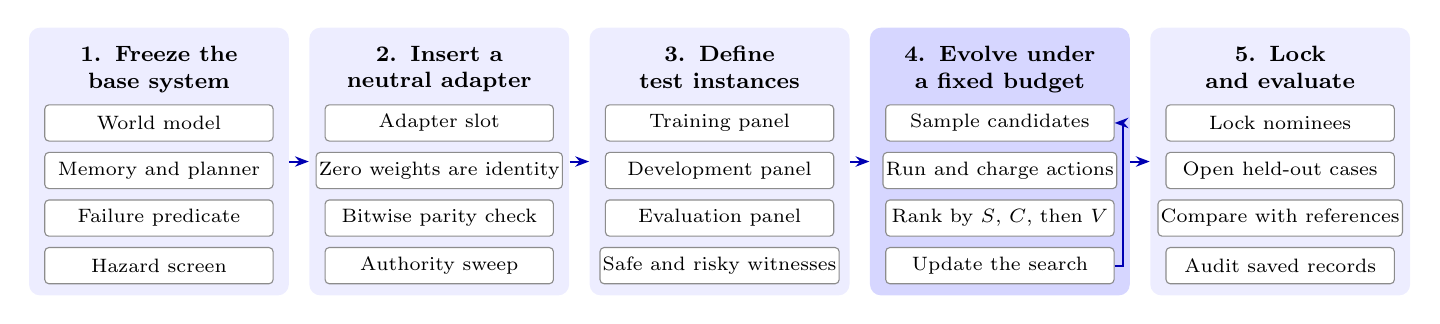
\begin{tikzpicture}[
  font=\footnotesize, >={Stealth[length=5pt]},
  panel/.style={draw=none, fill=blue!7, rounded corners=4pt, minimum width=33mm, minimum height=34mm, anchor=north west},
  evolved/.style={panel, fill=blue!16},
  head/.style={font=\footnotesize\bfseries, align=center, text width=31mm, anchor=north},
  item/.style={draw=black!45, fill=white, rounded corners=1.5pt, minimum width=29mm, minimum height=4.6mm, inner sep=1pt, font=\scriptsize, anchor=north},
  flow/.style={->, draw=blue!70!black, line width=0.7pt}]
  \foreach \i/\style/\title/\a/\b/\c/\d in {
    0/panel/{1. Freeze the\\base system}/World model/Memory and planner/Failure predicate/Hazard screen,
    1/panel/{2. Insert a\\neutral adapter}/Adapter slot/Zero weights are identity/Bitwise parity check/Authority sweep,
    2/panel/{3. Define\\test instances}/Training panel/Development panel/Evaluation panel/Safe and risky witnesses,
    3/evolved/{4. Evolve under\\a fixed budget}/Sample candidates/Run and charge actions/{Rank by $S$, $C$, then $V$}/Update the search,
    4/panel/{5. Lock\\and evaluate}/Lock nominees/Open held-out cases/Compare with references/Audit saved records} {
    \node[\style] (p\i) at (\i*35.6mm,0) {};
    \node[head] (h\i) at ($(p\i.north)+(0,-1.2mm)$) {\title};
    \node[item] (a\i) at ($(p\i.north)+(0,-9.8mm)$) {\a};
    \node[item] (b\i) at ($(a\i.south)+(0,-1.3mm)$) {\b};
    \node[item] (c\i) at ($(b\i.south)+(0,-1.3mm)$) {\c};
    \node[item] (d\i) at ($(c\i.south)+(0,-1.3mm)$) {\d};
  }
  \foreach \i/\j in {0/1,1/2,2/3,3/4}
    \draw[flow] (p\i.east) -- (p\j.west);
  \draw[flow] (d3.east) -- ++(1.1mm,0) |- (a3.east);
\end{tikzpicture}
\caption{Proposed framework for neutral-start adapter evolution around a frozen planner.}
\Description{Five panels in a row joined by arrows. Panel one freezes the world model,
memory and planner, failure predicate, and hazard screen. Panel two inserts a neutral adapter
with a parity check and authority sweep. Panel three defines training, development, and
evaluation panels with safe and risky witnesses. Panel four loops through sampling,
charged runs, lexicographic ranking, and search updates. Panel five locks nominees, opens
held-out cases, compares with references, and audits saved records.}
\label{fig:framework}
\end{figure*}

\textbf{1. Freeze the base system.} The world model, memory, planner settings, and failure
definition are fixed first. A task is admitted only if the bare planner both finishes and fails on
screened cases, since otherwise an adapter has nothing to show.

\textbf{2. Insert a neutral adapter.} The adapter may edit the planner's action or act inside its
final choice. Its one hard requirement is that zero means ``do nothing'', which we check exactly
before training. A sweep of random weights then shows whether the slot can move outcomes at all.

\textbf{3. Define test instances.} Training, development, and evaluation cases are frozen
separately. A passive monitor counts violations and never prevents them. Each evaluation case has
a scripted safe route and a scripted risky route, which must behave as declared before training.
If one does not, the study stops rather than replacing the case.

\textbf{4. Evolve under a fixed budget.} For a candidate's episodes $\tau_i$, we count
\begin{equation}
  \textstyle
  S=\sum_i \ind[g(\tau_i) \wedge \neg v(\tau_i)],\;
  C=\sum_i \ind[g(\tau_i)],\;
  V=\sum_i \ind[v(\tau_i)]
  \label{eq:counts}
\end{equation}
and rank by $S$, then $C$, then fewer $V$, encoded as
\begin{equation}
  F(\theta) = 81\,S(\theta) + 9\,C(\theta) - V(\theta).
  \label{eq:fitness}
\end{equation}
With at most eight episodes per candidate, these constants exactly reproduce that order, so they
are not tuned weights. Ranking on $S$ first targets what we want. Ranking on $C$ next stops a
controller that stands still, which never violates, from outranking one that finishes.
Equation~\ref{eq:fitness} still needs a definition of violation and of the task; what it removes
is the safety multiplier. Every action is charged to the search, so a method gains nothing by
finishing early.

\textbf{5. Lock and evaluate.} Nominees are locked before any evaluation case is opened. Each is
compared on the same cases with the bare planner and with an \emph{untrained} adapter, a random
draw with no selection, which shows how much of any change needs no search.

\begin{algorithm}[t]
\caption{Neutral-start adapter evolution}
\label{alg:search}
\small
\begin{algorithmic}[1]
\Require frozen planner $\pi_0$, neutral weights $\theta_0$, scales $s$, training and held-out cases, budget $B$
\State Check that $\theta_0$ reproduces $\pi_0$ exactly.
\State Set the search mean to zero: the bare planner.
\While{actions remain in $B$}
  \State Sample a population of candidates $x$.
  \For{each candidate $x$}
    \State Decode $\theta=\theta_0+s\odot x$.
    \State Run $\pi_\theta$ on the training cases, charging every action.
    \State If all its episodes ran, score it with Equation~\ref{eq:fitness}.
    \State If the budget cut it short, keep it on record, unscored.
  \EndFor
  \If{every candidate was scored}
    \State Update the search in sampling order, keeping ties equal.
  \EndIf
\EndWhile
\State Lock the nominee.
\State Only now open the held-out cases.
\State Compare it with the bare planner and an untrained draw.
\end{algorithmic}
\end{algorithm}

\section{Experimentation}
\label{sec:design}

Our experiments address four research questions. RQ1: does a neutral-start evolved adapter raise
safe completion on cases that search has not seen? RQ2: which parts of the framework carry the
effect: the search space, the safety-aware ranking, the hazard inputs, or the recurrent state? RQ3:
how does evolution compare with PPO at the same budget? RQ4: does the framework carry over to a
simulated manipulation task?

\subsection{Test systems}
\label{sec:systems}

\textbf{TwoRoom.} A body must reach a goal image's position within 200 actions, in an arena with
one wall and one door. AP's memory holds observations from 8,000 dataset episodes. Retrieval
matches the pair (current image, goal image), and the anchor is the observation five steps after
the match. $\mathcal{A}_t$ is searched by one-block CEM with 300 candidates, 30 iterations, and 30
elites. % src: results/05-anchored-planning.md; experiments/scripts/replication_worker.py
A supplied circle gives an exclusion radius of 18 around the body's center. The planner cannot see
this hazard, because it is absent from the images. Only the adapter and the monitor receive it.
% src: results/06-hazard-qualification.md, 07-hazard-screen.md
In a screen of 12 layouts, bare AP qualified on open rooms (6/8 completed, 4/8 violated) and
wall-constrained rooms (6/8, 6/8) and failed on doorways (0/8 completed), so every result here is a
same-room task. Eight admitted layouts form the training panel, where the bare planner scores 1/8
safe, 7/8 complete, and 6/8 violated. % src: results/08-recurrent-adapter-pilot.md

\begin{figure}[t]
\centering
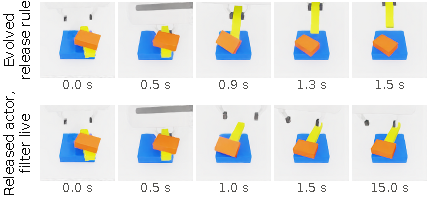
\includegraphics[width=\columnwidth]{figures/block_frames.pdf}
\caption{Block Plucking from the front camera, on one start of the regular task, in recorded runs
from an earlier study (not pilot episodes). An evolved release rule draws out the yellow middle
block by 1.5\,s. The released actor with its filter live does not, and times out at 15\,s.}
\Description{Two rows of five camera frames showing a blue base, a yellow middle block, and
an orange top block, with a gripper above. In the upper row the gripper draws the yellow block
out and the orange block settles on the blue base by 1.5 seconds. In the lower row the yellow
block stays wedged under the orange block, unchanged from 1.5 to 15 seconds.}
\label{fig:blockframes}
% src: archive/20261022/runs/unisafe/videos-20261019/recordings/{evolution,frozen}, seed 1000
\end{figure}

\textbf{Block Plucking.} A simulated Franka arm must pull the middle block from a three-block stack
(Figure~\ref{fig:blockframes}), in Isaac Sim 6.2 and Isaac Lab 3.0 at 20\,Hz. We use the Hard variant,
with a lighter top block and smaller base. A violation is, at any control, a block below 0.13\,m, the
top block more than 0.07\,m from the base, or the gripper leaving the boundary. Sustained success
means success still holds 40 controls later with no violation, and here $S$ counts sustained safe
success. These are the task's own predicates, so no hazard is invented.
% src: SafeBlock/Stage1.md section 1; SafeBlock/Probes.md
AP's memory is the 161,709 steps of the 1,369 success-only demonstrations released with UNISafe.
Retrieval returns the 64 nearest steps, the anchor is the feature five steps after the nearest, and
$\mathcal{A}_t$ holds the five recorded actions after each retrieved step. UNISafe's filter stays in
shadow mode in every planner condition, so its signals are logged and never applied. In probes on
the regular task, this planner completed 7 of 8 episodes, against 1 of 8 for the released actor. On
Hard it completed 5 of 12 and violated in 8 of 12, so completion and risk are in tension.
% src: SafeBlock/ProbeResults.md Probe A and Probe B; any-control counts recounted from summaries
Each episode needs a fresh simulator process, because in-process resets diverged within the first few
controls. A median episode takes 25\,s rather than 6\,s. % src: SafeBlock/Stage1Results.md

\subsection{Adapters}

\textbf{Gain and residual (TwoRoom).} A small recurrent network reads the planner's action $b_t$ and
returns a gain and a correction:
\begin{equation}
  a_t = \operatorname{clip}\bigl((1+\tanh v_t)\odot b_t + \tanh u_t,\,-1,\,1\bigr),
  \label{eq:gain}
\end{equation}
where $(v_t,u_t)$ come from a linear head on a 32-unit GRU above a 32-unit tanh layer: 19,172 weights
in all, of which the head holds the last 132. The 396 inputs include the embeddings, position, the
hazard's relative position and radius, and recent actions. % src: SafeLeWM/AdapterPilot.md
No true goal coordinates or outcome flags reach the network. The head starts at zero, so
$a_t=b_t$. Clipping is the legal action range, not a safety filter.

\textbf{Segment selector (Block Plucking).} Five weights $w$ re-rank the 64 retrieved segments inside
the planner's final choice. With $c_i$ the planner's imagined cost for segment $i$ from
Equation~\ref{eq:plan} and $y_i$ its standardized features,
\begin{equation}
  i^\star = \arg\min_{i}\;\bigl(c_i - w^{\top} y_i\bigr).
  \label{eq:select}
\end{equation}
The features are retrieval distance, imagined cost, mean arm-action size, the fraction of closing
gripper commands, and progress through the demonstration. With $w=0$ the planner is unchanged. A
selector can only replay recorded behavior, which limits both its reach and its damage.

\subsection{Search and studies}

We use diagonal \cmaes{}~\cite{ros2008simple} from pycma 4.4.4 with cumulative step-size adaptation,
population 8, and initial step size 0.5. In Algorithm~\ref{alg:search}, $s$ holds fan-in scales on
TwoRoom and ones on Block Plucking. Random search draws from the same initial distribution,
$N(0,0.5^2 I)$. \emph{Native} is the bare planner. Our first pilot was stopped because pycma's default
step-size rule at this dimension clashed with our tie-breaking. We set the rule explicitly and
excluded those 459 episodes from every comparison. % src: SafeLeWM/AdapterPilotCorrection.md

On TwoRoom, each candidate runs on all eight training layouts, and the nominee is the best complete
candidate, earliest on exact ties. Replication and later searches each get exactly 40,000 actions.
That buys 34 to 44 candidates but only 4 or 5 \cmaes{} updates, which is closer to sharpened sampling
than to long evolution.

PPO~\cite{schulman2017ppo} uses the same actor, the head coordinates, and the same 40,000 actions. Each
episode receives $U=(81S+9C-V)/90$, the single-episode form of Equation~\ref{eq:fitness}. In expectation
these constants act as weights, so PPO optimizes a fixed scalarization, not the order that search
sees. Settings were frozen with no sweep: learning rate $3\times10^{-4}$, ratio clip 0.2, 4 epochs,
minibatches of 4 episodes, $\lambda=0.95$, and $\gamma=1$. % src: SafeLeWM/MatchedPPO.md

The TwoRoom studies ran in sequence with fresh seeds. A \emph{pilot} used one repeat and four new
layouts. A \emph{replication} used three repeats and twelve new layouts with three planner seeds each.
A \emph{mechanism study} then had two stages. Stage~A compared three search spaces, using the
replication layouts as development data: all 19,172 weights (\emph{full}), the 132 head coordinates
(\emph{head}), and 256 coefficients of a random projection (\emph{subspace}). Stage~B retrained in the
winner with five arms over three repeats: \emph{main} (safety-aware \cmaes{}), \emph{random},
\emph{task} (\cmaes{} ranked by completions alone), \emph{blind} (hazard inputs zeroed), and
\emph{reset} (GRU state cleared before every action). All 15 nominees were evaluated on 24 new layouts,
twelve open and twelve wall-constrained, with three planner seeds each. % src: SafeLeWM/AdapterMechanism.md
The \emph{rerun} repeated head-space \cmaes{} and random search with PPO, from fresh seeds, on those
24 layouts.

On Block Plucking, \cmaes{} ran 8 generations of 8 candidates on two shared starts per generation, and
random search ran 16 draws on 8 starts, 128 episodes each. The \cmaes{} nominee here is the final
distribution mean, never itself evaluated in training, and the random nominee is the top-scoring draw.
Each of three repeats has 16 fresh starts. Verdict rules were
written first. On one repeat, the framework \emph{transfers} if \cmaes{} gains at least 3 sustained
successes on native with no more violations, and shows \emph{no signal} if both differences are within
1. On 48 pooled starts those thresholds become 9 and 3. Anything else is \emph{mixed}. % src: SafeBlock/Pilot.md

On TwoRoom, a crossed cluster bootstrap (2,000 draws) resamples repeats and layouts. With three repeats
these intervals are exploratory, so we claim no difference as significant. On Block Plucking we report
Wilson intervals, and McNemar's exact test as a description only. Zero weights reproduced the bare
planner exactly on both systems. A separate auditor checked all 13,679 mechanism and PPO episodes. Two
audits first failed on a timestamp check; we kept those failures on record, corrected the check, and all
passed with no episodes rerun. % src: results/12-audit-amendment.json, ppo 4090-audit.json, l4-audit.json

\section{Results}
\label{sec:results}

All counts are safe completions unless stated otherwise, and outcomes overlap.

\subsection{Results for TwoRoom}

\begin{figure}[t]
\centering
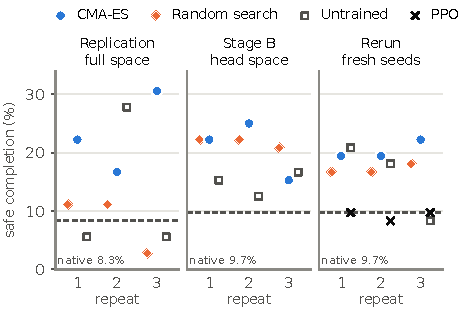
\includegraphics[width=\columnwidth]{figures/headline.pdf}
\caption{Every held-out TwoRoom search, repeat by repeat. Dashed lines mark native on that panel.
Panels differ in layouts or search space.}
\Description{Three panels of safe completion percentage by repeat. Blue CMA-ES dots sit above
the dashed native line in all nine repeats, between about 15 and 31 percent, against native at
8.3 and 9.7 percent. Orange random search diamonds sit above the line in eight of nine, and
hollow untrained squares in six of nine. Black PPO crosses in the third panel sit on or just
below the line.}
\label{fig:headline}
\end{figure}

\begin{table}[t]
\caption{Safe completion (\%) on held-out layouts, pooled over three repeats, with the number of
searches above native.}
\label{tab:headline}
\small
\setlength{\tabcolsep}{4.5pt}
\begin{tabular}{@{}lcccc@{}}
\toprule
Controller & Replication & Stage~B & Rerun & Above native \\
\midrule
\textbf{\cmaes{}} & \textbf{23.1} & \textbf{20.8} & \textbf{20.4} & \textbf{9/9} \\
Random search & 8.3 & 21.8 & 17.1 & 8/9 \\
Untrained & 13.0 & 14.8 & 15.7 & 6/9 \\
PPO & -- & -- & 9.3 & 0/3 \\
Native & 8.3 & 9.7 & 9.7 & -- \\
\bottomrule
\end{tabular}
% src: results/09, 12, 14: 25,9,14 of 108, native 3/36; 45,47,32 of 216, native 7/72; 44,37,34,20 of 216, native 14/144
\end{table}

\cmaes{} scored above the bare planner in all nine held-out searches (Figure~\ref{fig:headline} and
Table~\ref{tab:headline}). It reached 23.1\%, 20.8\%, and 20.4\% safe completion against 8.3\%, 9.7\%,
and 9.7\%, which is two to nearly three times native's rate. It scored above random search in seven of
nine repeats, equal in one and below in one, and above unselected draws in six of nine. Summed over the
nine searches, a post hoc total on panels that are not independent, it reached 114 of 540, against 93
for random search and 80 for unselected draws. Random search also scored above native in eight of nine
searches, and unselected draws in six, so part of the gain needs no search. Every exploratory interval
below includes zero.

\begin{figure}[t]
\centering
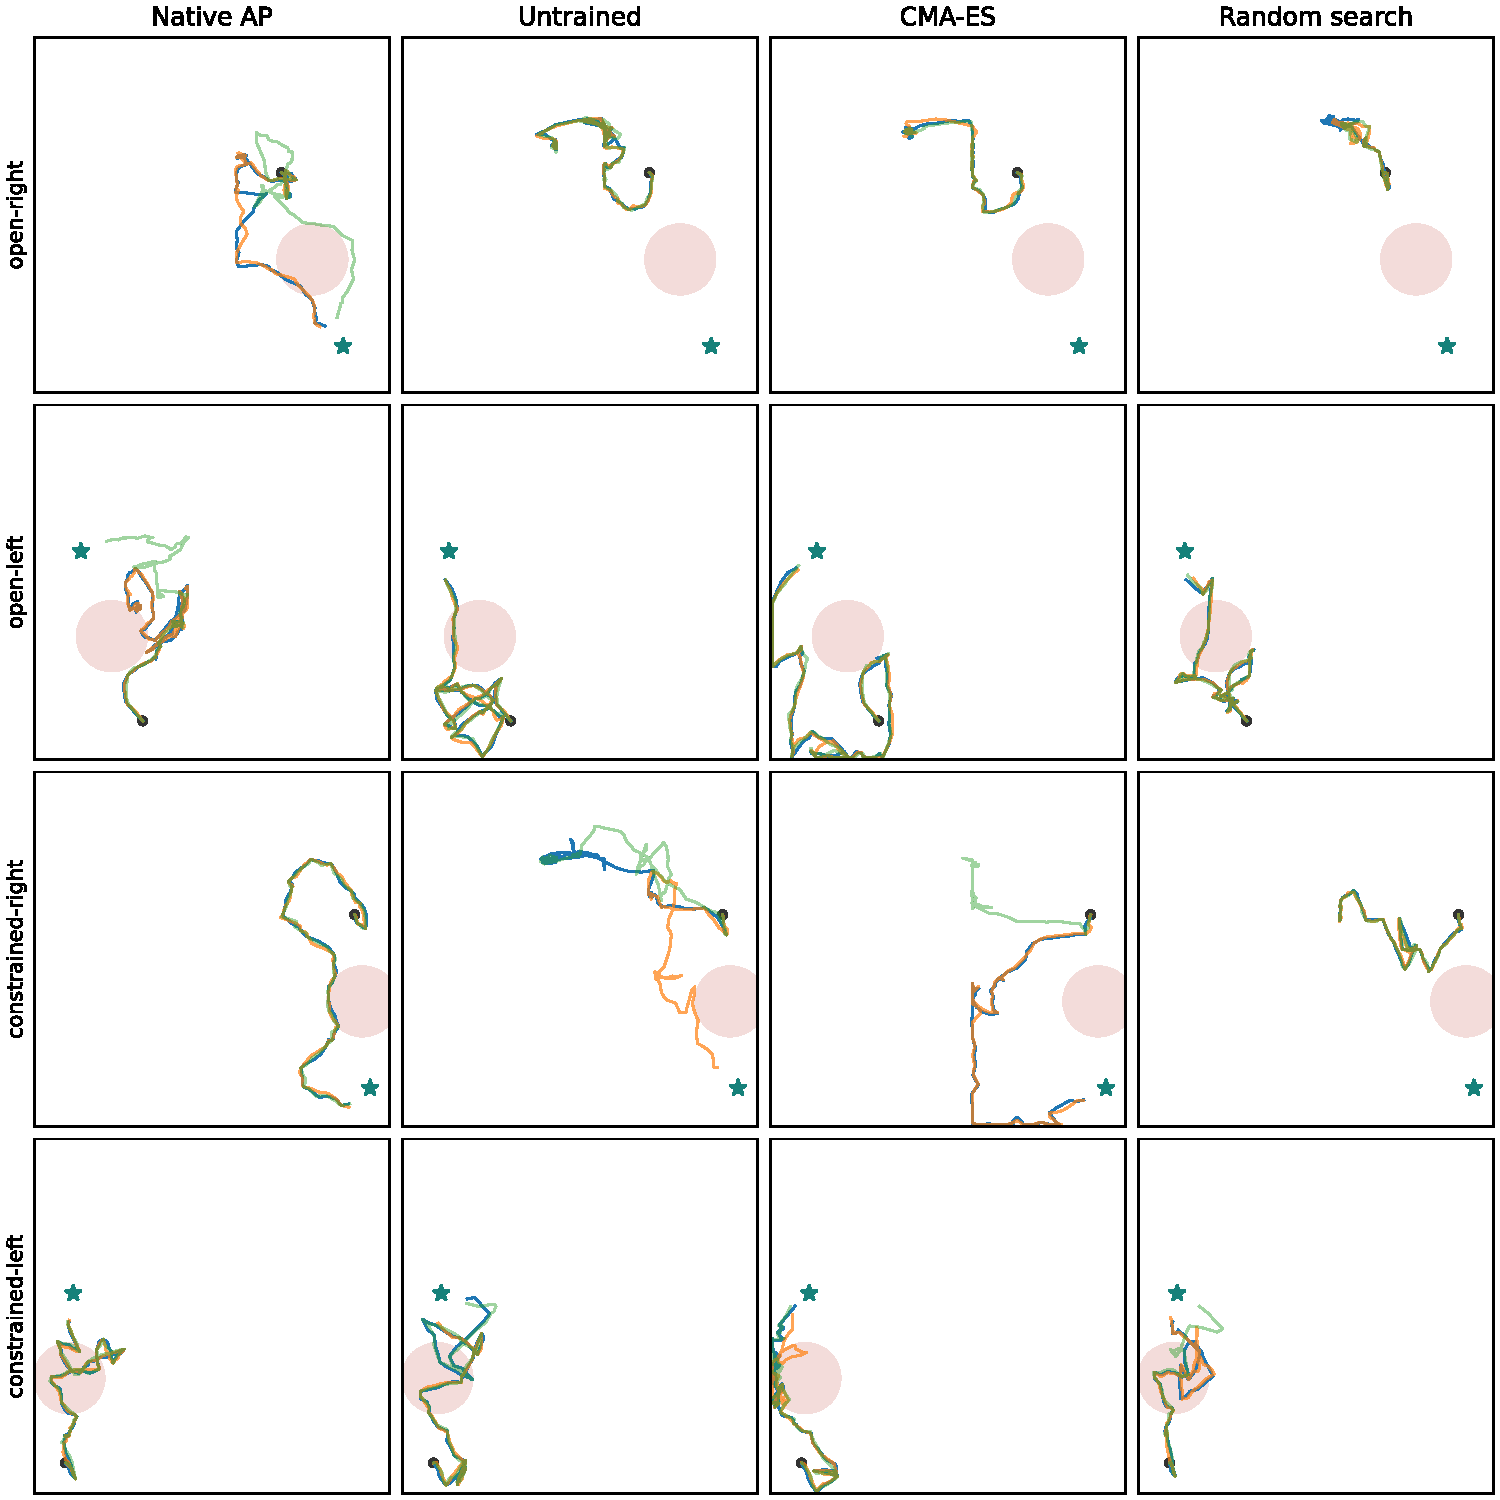
\includegraphics[width=\columnwidth,trim=0 352 0 0,clip]{figures/trajectories.pdf}
\caption{Pilot trajectories, one line per planner seed. The circle is the exclusion zone and the star
the goal. On open-left, \cmaes{} detours and completes safely in all three seeds. On open-right, it
moves away from the goal and does not finish, with no violation.}
\Description{A grid of two rows and four columns of trajectory plots for native AP,
untrained, CMA-ES and random search. In the lower row CMA-ES routes around the circular
exclusion zone to the goal. In the upper row it moves away from the goal.}
\label{fig:traj}
\end{figure}

The pilot gave the first signal. On four new layouts, \cmaes{} reached 5/12, against 2/12 native, 1/12
untrained, and 0/12 for selected random search, with 3/12 violations against native's 10/12 and 8/12
completions against 10/12. Equal caps did not equalize work here: \cmaes{} used 36,366 actions against
random search's 32,182. % src: SafeLeWM/results/08-recurrent-adapter-pilot.md
Figure~\ref{fig:traj} shows a detour around the exclusion zone on one layout and an unfinished
trajectory on another. The mean correction was 0.303 in normalized action units, so the adapter was
using real authority.

The replication kept the direction in the full 19,172-dimensional space. \cmaes{} reached 8, 6, and 11
of 36, against native's 3 and random search's 4, 4, and 1. The differences were +14.8 points against
native [$-$12.0, +39.8] and +14.8 against random search [$-$3.7, +36.1]. One unselected draw scored above
its paired \cmaes{} run. All three of native's safe completions came from one layout where every \cmaes{}
repeat scored zero, so gains came with some lost competence. Stage~A reran this configuration on the
same layouts with new seeds and scored 15/108 against 25/108, or 40/216 (18.5\%) together, so the +14.8
should be read with care. % src: SafeLeWM/results/09-adapter-replication.md

\begin{table}[t]
\caption{Stage~B outcomes on 24 layouts. The last column gives main minus the arm in percentage points
of safe completion, with exploratory 95\% intervals.}
\label{tab:outcomes}
\footnotesize
\setlength{\tabcolsep}{3.5pt}
\begin{tabular}{@{}lccccc@{}}
\toprule
Arm & Safe by repeat & Safe & Compl. & Viol. & Difference \\
\midrule
Native & 7 (shared) & 7/72 & 39/72 & 39/72 & +11.1 [$-$7.4, +27.3] \\
Untrained & 11, 9, 12 & 32 & 130 & 114 & +6.0 [$-$9.7, +21.3] \\
Random & 16, 16, 15 & 47 & 134 & 95 & $-$0.9 [$-$16.7, +15.3] \\
Task & 4, 18, 7 & 29 & 123 & 120 & +7.4 [$-$4.6, +23.6] \\
Blind & 6, 16, 14 & 36 & 125 & 107 & +4.2 [$-$6.9, +18.1] \\
Reset & 15, 13, 9 & 37 & 136 & 111 & +3.7 [$-$12.5, +19.0] \\
Main & 16, 18, 11 & \textbf{45} & 115 & 94 & -- \\
\bottomrule
\end{tabular}
% src: SafeLeWM/results/12-adapter-mechanism.md
\end{table}

In Stage~B, the main arm reached 45/216 safe completions (20.8\%) on 24 new layouts against native's 7/72
(9.7\%, Table~\ref{tab:outcomes}), and it scored above native in every repeat. Unselected draws reached
14.8\%, so about half of that gap needs no search. Pooled completion was similar (53.2\% against 54.2\%)
and pooled violations were lower (43.5\% against 54.2\%), with no interval computed for either. These
pools hide variation. Main's completions were 36, 49, and 30 of 72 against native's 39, and its violations
29, 39, and 26. Violations fell in open rooms (16.7\% against 41.7\%), where completion also fell (37.0\%
against 47.2\%), and not on wall-constrained layouts (70.4\% against 66.7\%). This fall did not repeat with
fresh seeds (Section~\ref{sec:rq3}). % src: mechanism summary.json

\begin{figure}[t]
\centering
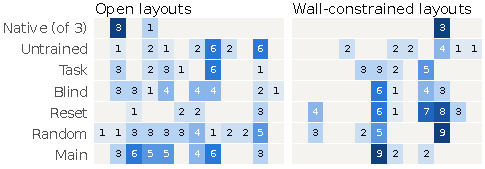
\includegraphics[width=\columnwidth]{figures/layouts.pdf}
\caption{Stage~B safe completions per layout, out of 9 episodes, or 3 for native. Blank cells are zero.}
\Description{A heat map with 24 layouts as columns and seven arms as rows, split into
open and wall-constrained groups. Safe completions cluster on a few columns, and
different arms succeed on different columns. Main reaches 9 of 9 on one wall-constrained
layout and Random reaches 9 of 9 on another, the one native solves. Many cells are zero.}
\label{fig:layouts}
\end{figure}

The gains are uneven across layouts (Figure~\ref{fig:layouts}). Main's safe completions fell on 10 of 24
layouts, and 21 of its 45 came from just three. Of the 45, 37 came on layouts where native had none. Some
competence was lost: on the two layouts native solved in all three seeds, main managed 3/9 and 0/9, and
random search 1/9 and 9/9. Layouts spread far more than arms do, with a standard deviation of 1.42 safe
completions of nine against 0.27.
% src: Oracle/figures/data.json layouts, population sd of layout means and of arm means

\subsection{Results for the mechanism study}

Stage~A chose the search space. Full, head, and subspace reached 15, 27, and 18 of 108. Head won under the
frozen rule, but one search decided it: repeat A2 gave head 16/36, and without A2 head would rank last, at
11/72 against 14/72 and 15/72. We therefore treat head as a workable configuration, not as the better
search space.

Main versus random changes only how candidates are proposed. They scored 45 and 47, and the interval is
far too wide to call them equal. Main versus task removes safety from the ranking: task scored 29 with 120
violations, against main's 45 and 94. One repeat needs care. All \cmaes{} arms in a repeat share their first
population, and in B1 main and task chose the same first-generation candidate, so their difference there
is zero by construction. In a post hoc look at the other two repeats, main scored 27/144 against task's
11/144. % src: selection-b.json; parameters compared directly, main==task in B1
No Stage~B contrast excludes zero, and one panel cannot rank selection against search in general.

Both main and random end training at four or five of eight safe completions, though main leads for much
of the budget in two repeats. In one of three main searches, and three of nine safety-ranked \cmaes{} arms,
the nominee came from the first generation, before any update, which is exactly what random search does.
% src: mechanism summary.json, generation field

Blind scored 36/216, and in B1 it has the same weights as main. When we moved the hazard on eight base
layouts, blind's actions stayed identical in 72/72 pairs and main's changed in 72/72, so the hazard inputs do
reach behavior. Yet safe completions rose similarly, from 11 to 18 for main and from 9 to 17 for blind, so we
cannot credit that rise to hazard awareness. Reset scored 37/216, with 8/108 in open rooms and 29/108 on
wall-constrained layouts, where main had 32/108 and 13/108. This crossing was not planned, so it is a lead
for later work, not a result.

\subsection{Results for PPO}
\label{sec:rq3}

\begin{table}[t]
\caption{PPO comparison on the Stage~B layouts, with R0 and R1 on an RTX 4090 and R2 on an L4. Ranges cover
repeats. Distance is the nominee's L2 norm from neutral, Correction the mean action change per episode, and
Same the episodes of 72 with native's outcome.}
\label{tab:ppo}
\small
\setlength{\tabcolsep}{3pt}
\begin{tabular}{@{}lcccrr@{}}
\toprule
Controller & Distance & Correction & Same & Safe by repeat & Total \\
\midrule
PPO & 0.04--0.10 & 0.003--0.006 & 59--64 & 7, 6, 7 & 20/216 \\
Random search & 5.87--6.08 & 0.22--0.29 & 29--38 & 12, 12, 13 & 37/216 \\
\cmaes{} & 7.97--8.81 & 0.24--0.32 & 23--28 & 14, 14, 16 & 44/216 \\
Untrained & 5.50--6.06 & 0.17--0.31 & 25--40 & 15, 13, 6 & 34/216 \\
Native & 0 & 0 & -- & 7 per host & 14/144 \\
\bottomrule
\end{tabular}
% src: SafeLeWM/results/14-matched-ppo.md; outputs/ppo-20261101/{4090,l4}-summary.json, combined-analysis.json;
% nominee genotypes from archive/evidence/ppo-{4090,l4}-20261101.tar.gz
\end{table}

PPO stayed close to the bare planner (Table~\ref{tab:ppo}). It reached 9.3\% safe completion against native's
9.7\%, with 50.9\% completion and 53.7\% violations against 53.5\% and 52.1\%. The reason is simple arithmetic.
Its 40,000 actions bought 10 updates and 292 to 300 Adam steps. At a learning rate of $3\times10^{-4}$, that
moves each coordinate by at most about 0.09, whereas the first \cmaes{} population already samples with a
standard deviation of 0.5. Its nominees stayed within 0.10 of neutral. Reaching \cmaes{}'s distance would take
at least 8 times the learning rate, and about 60 to 80 times at the efficiency observed. Reward only at the end
of an episode may be a second obstacle, which we did not measure.
% derivation: 300 x 3e-4 = 0.09 per coordinate at most; largest CMA nominee rms 0.77 / 0.09 = 8.5;
% L2 ratios of CMA nominee to final PPO policy: 8.07/0.109, 8.81/0.111, 7.97/0.129 = 74, 79, 62
So the \cmaes{} gap over PPO, +11.1 points [$-$6.9, +28.2], is really a gap over native, and it says nothing
general about reinforcement learning. We kept the frozen settings as the protocol required and report this
as a flaw in the comparison.

The rerun also gives a second look at Stage~B. It used the same layouts, so it is not an independent
replication, but it shows what held. \cmaes{} scored 44/216 against Stage~B's 45/216, and unselected draws
34/216 against 32/216. Random search scored 37/216 against 47/216, and \cmaes{} led it in all three repeats, by
+3.2 points overall [$-$11.6, +18.5]. Violations did not hold: \cmaes{} violated in 50.5\% of episodes against
native's 52.1\%, while random search reached 38.9\% with completion down to 45.8\%. So the gain in safe
completion over native repeated, and the fall in violations did not.

\subsection{Results for Block Plucking}
\label{sec:block}

On 48 fresh Hard starts, the bare planner violated at a rate of 0.52 (Wilson 95\% interval 0.38 to 0.66),
succeeded at 0.58, and sustained success at only 0.29. It cannot see the success predicate, so it keeps
following anchors after the block is out. % src: SafeBlock/Stage1Results.md Calibration; ProbeResults.md

Before any search, we compared two interfaces with 24 random genotypes over 4 starts. A bounded residual on the
planner's command, a 279-weight feed-forward network, was destructive at both bounds tested: it completed 1
of 96 episodes and violated in 85. The segment selector completed 76 of 96 and violated in 18. All four starts
were easy for the bare planner, which completed them with no violation, so the selector was still worse than
the base here. Neither interface passed the frozen gate, which required outcomes to move both ways. We did not
run its fallback of a wider residual, which pointed the wrong way, nor a proposed test at bound 0.1. Choosing
the selector was a later, recorded decision, and no optimizer ran on the residual, so this compares random
adapters only. % src: SafeBlock/Stage1Results.md; Stage1.md amendment; Pilot.md

\begin{figure}[t]
\centering
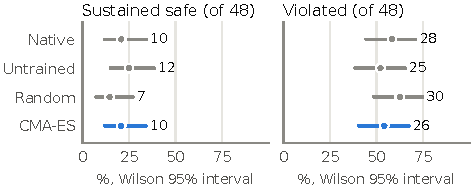
\includegraphics[width=0.88\columnwidth]{figures/block.pdf}
\caption{Block Plucking pilot on 48 fresh starts over three repeats.}
\Description{Two dot plots with Wilson intervals. Sustained safe success: Native 10,
Untrained 12, Random 7, CMA-ES 10 of 48. Violated: Native 28, Untrained 25, Random 30,
CMA-ES 26 of 48. All intervals overlap.}
\label{fig:block}
\end{figure}

Figure~\ref{fig:block} summarizes the pilot. Repeats 0 and 1 each read ``mixed'': \cmaes{} gained two sustained
successes on native and removed two violations, short of the threshold of three. Repeat 2 went the other way,
with four fewer sustained successes and two more violations. Pooled over 48 starts, \cmaes{} and native each
reached 10 sustained successes, with 26 violations against 28, which the rule calls \emph{no signal}. Paired by
start, \cmaes{} gained 9 and lost 9 (McNemar exact $p=1.00$, descriptive only). Three unselected draws scored
12 and 25, and selected random search 7 and 30, both also no signal. The three nominees' weights disagree, so we
offer no behavioral reading of them. Overall, this pilot gives no evidence that the framework transfers to this
task. % src: SafeBlock/PilotResults.md, PilotPooled.md

\section{Discussion}
\label{sec:discussion}

The main result is that evolved adapters are a usable lever on TwoRoom. All nine held-out \cmaes{} searches
scored above native. Including the development searches of Stage~A, 16 of 18 did, with one matching it and one
below. On the 24 layouts the total barely moved with fresh seeds. Part of this lever needs no search, since 6 of 9
unselected draws also scored above native. Yet tiny changes were not enough: PPO's corrections left safe
completion at 7, 6, and 7. It seems the planner must be disturbed by enough, and search adds to that, since
\cmaes{} led the post hoc totals. % src: replication 3, Stage A 9, Stage B main 3, rerun main 3; native 3/36 and 7/72

The comparison with sampling favors \cmaes{} on TwoRoom but is not settled. It led random search by 25 to 9 in
the full space, and scored 45 against 47 and then 44 against 37 in the head space. On Block Plucking, where
nominee rules differ, it led 10 to 7 of 48, though two of three repeats are ties by the rule. With four or
five updates, \cmaes{} has little chance to move from exploration to exploitation, so these comparisons may
change at a larger budget.

Noise was as large as the gaps between search methods. Task scored 4, 18, and 7 of 72 across repeats, head 6,
5, and 16 of 36, and unselected draws 2, 10, and 2 of 36, so one arm moved by 19 to 31 points, while the largest
pooled gap between search methods was 14.8. A pool averages three repeats, so these are not the same kind of
number, but three repeats cannot average away swings that size. Selection adds to this. The 12 safety-ranked
Stage~B nominees fell from 52\% safe on training layouts to 19\% on new ones, partly winner's curse from taking
the best of about 40. Outcomes also move easily: PPO's corrections of 0.006 or less changed 8 to 13 of 72
outcomes, and moving native between GPU types changed 4 of 72. Larger selection panels may therefore be worth
more than further generations.

Block Plucking shows the limits of reuse. Neutral start, diagonal \cmaes{}, ordered fitness, parity checks, and
locked nominees all carried over, but the adapter, budget, training panel, and nominee rule all changed, so we
claim reuse of a procedure, not of weights. An earlier study on the regular task is relevant
(Figure~\ref{fig:blockframes}). The released actor with its filter live completed only 2 or 3 of 64 reserved
starts, a hand-designed release delay 55/64, an evolved version of that rule 54/64, and random search over the
same rule 56/64. % src: SafeBlock/BlockPlucking.md, record table
Once a good lever existed, the optimizer had little left to do. The open question is whether search can find
the lever without being handed it.

Step 1 of the framework also proved a real gate. On PushT, AP reached 15/50, below our frozen readiness rule of
20, which we waived, and on OGBench Cube~\cite{park2025ogbench} it reached 26/50, yet with hazards it completed
0/16. We trained no adapter on either, and a later PushT screen failed its prerequisite gate.
% src: SafeLeWM/results/10-pusht-screen.md, 11-cube-screen.md, 13-pusht-authority.md

\section{Conclusions}
\label{sec:conclusions}

We proposed a framework for evolving safety adapters around frozen world-model planners, stated as a relaxed
CMDP. On held-out TwoRoom layouts, \cmaes{} adapters scored above the bare planner in all nine searches, at about
twice its safe completion, and above random search in seven of nine repeats. The gain repeated with fresh seeds,
a fall in violations did not, and part of the gain needs no search. On Block Plucking, the pilot showed no signal
over 48 starts.

These results have limits. Layouts are constructed, not sampled, and each is new to adapter search but not
necessarily to model pretraining. Planner seeds on a layout are correlated, so 216 episodes are not 216 independent
tasks. Three repeats make intervals exploratory, with no correction across contrasts, and a wide interval is not
equivalence. One PPO repeat ran on different hardware. Stage~A reused the replication's layouts, so it is selection
evidence. On Block Plucking, each adapter was trained on few starts, and the world model and memory come from the
regular task, so Hard is out of distribution for both: the filter's signals fire on up to 79\% of planner controls
there. We did not compare with a tuned penalty or a hand-designed rule, so reduced tuning remains a hypothesis, and
this paper does not test a requested risk limit. Nothing here certifies safety: 44\% and 50\% of main-arm episodes on
the final layouts still violated.

Future work should select on larger panels, use enough repeats and budget to separate evolution from sampling, and
scale PPO to travel as far as \cmaes{}. Solving Equation~\ref{eq:cmdp} at a stated $\delta$ is the natural next step,
and noise makes it a real evolutionary problem. At the Block Plucking planner's violation rate and a limit of 0.25
with eight episodes, a candidate no safer than the bare planner still passes 12\% of the time, and one with half the
risk fails 35\% of the time. % src: SafeBlock/Stage1Results.md Calibration

\bibliographystyle{ACM-Reference-Format}
\bibliography{references}

\end{document}
